%%%%%%%%%%%%%%%%%%%%%%%%%%%%%%%%%%%%%%%%%%%%%%%%%%%%%%%%%%
\begin{frame}
  \begin{center}
    {\Large Introduction to TensorFlow Data}
	
	% {\tiny (Ref: Building a High-Performance Data Pipeline with Tensorflow 2.x - Mayank Kumar )}
  \end{center}
\end{frame}

%%%%%%%%%%%%%%%%%%%%%%%%%%%%%%%%%%%%%%%%%%%%%%%%%%%%%%%%%%%
\begin{frame}[fragile]\frametitle{Data Pipeline}
\begin{itemize}
\item Goal:  Having an efficient, scalable as well as generic pipeline 
\item Multiple sources, multiple formats (image, text, csv, server log file, videos, audio files, etc.)
\item Tensorflow  tf.data module can be easily customized to consume these data efficiently and send it to the model for further computations. 
\end{itemize}
\end{frame}

%%%%%%%%%%%%%%%%%%%%%%%%%%%%%%%%%%%%%%%%%%%%%%%%%%%%%%%%%%%
\begin{frame}[fragile]\frametitle{What ML needs from Data Pipeline}
\begin{itemize}
\item Machine learning models are data-hungry
\item Before data is fed to an ML model it should be:
\begin{itemize}
\item Shuffled
\item Batched 
\item Be available before the current epoch is finished
\end{itemize}
\end{itemize}

{\tiny (Ref: Building data pipelines with tf.data - Sayak Paul)}
\end{frame}

%%%%%%%%%%%%%%%%%%%%%%%%%%%%%%%%%%%%%%%%%%%%%%%%%%%%%%%%%%%
\begin{frame}[fragile]\frametitle{Tensorflow Data}
\begin{itemize}
\item  \lstinline|tf.data| module
\item \lstinline|tf.data.Dataset| abstraction that represents a sequence of elements, in which each element consists of one or more components, which can be used as a source to consume data.
\item E.g. a single element in spam classifier dataset has two components: a text data and its label 
\item \lstinline|tf.data.Dataset| behaves as a python iterator, which can be easily accessed using a python $for$ loop.
\end{itemize}
\end{frame}

%%%%%%%%%%%%%%%%%%%%%%%%%%%%%%%%%%%%%%%%%%%%%%%%%%%%%%%%%%
\begin{frame}
  \begin{center}
    {\Large Load Data}
	
	{\tiny (Ref: Building a High-Performance Data Pipeline with Tensorflow 2.x - Mayank Kumar )}
  \end{center}
\end{frame}

%%%%%%%%%%%%%%%%%%%%%%%%%%%%%%%%%%%%%%%%%%%%%%%%%%%%%%%%%%%
\begin{frame}[fragile]\frametitle{Tensorflow Ready Datasets}
\begin{lstlisting}
train, test = tf.keras.datasets.fashion_mnist.load_data()

images, labels = train
images = images/255

dataset = tf.data.Dataset.from_tensor_slices((images, labels))
\end{lstlisting}
\end{frame}

%%%%%%%%%%%%%%%%%%%%%%%%%%%%%%%%%%%%%%%%%%%%%%%%%%%%%%%%%%%
\begin{frame}[fragile]\frametitle{From Small CSV}
\lstinline|tf.data.Dataset.from_tensor_slices|

\begin{itemize}
\item CSV small enough to fit in memory.
\item Read it into Pandas dataframe
\item \lstinline|tf.data.Dataset.from_tensor_slices| to convert dataframe object to \lstinline|tf.data.Dataset|
\end{itemize}

\begin{lstlisting}
df = pd.read_csv("sample.csv")
dataset = tf.data.Dataset.from_tensor_slices(dict(df))
\end{lstlisting}
\end{frame}

%%%%%%%%%%%%%%%%%%%%%%%%%%%%%%%%%%%%%%%%%%%%%%%%%%%%%%%%%%%
\begin{frame}[fragile]\frametitle{From Python Generator}
\lstinline|tf.data.Dataset.from_generator|

\begin{itemize}
\item Uses python generators for consuming the dataset.
\item Can incorporate transformation logic on python side.
\item Transformation happens on-the-go during data consumption.
\end{itemize}

\begin{lstlisting}
def read_csv(filepath,skip_rows):
	with open(filepath,'r') as csvfile:
		data = csv.reader(csvfile, delimiter=",")
		for index, row in enumerate(data):
			if index < skip_rows:
				continue
			yield row[0],row[1],row[2]
			
dataset = tf.data.Dataset.from_generator(read_csv, output_types =(tf.string,
																					tf.int8,tf.float16)
\end{lstlisting}
\end{frame}

%%%%%%%%%%%%%%%%%%%%%%%%%%%%%%%%%%%%%%%%%%%%%%%%%%%%%%%%%%%
\begin{frame}[fragile]\frametitle{From CSV}
\lstinline|tf.data.experimental.make_csv_dataset|

\begin{itemize}
\item Batch-wise loading
\item Shuffling possible
\end{itemize}

\begin{lstlisting}
path = tf.keras.utils.get_file(filepath)
dataset = tf.data.Dataset.make_csv_dataset(path,batch_size=32,
																						label_name = target_column,
																						select_columns=feature-columns,
																						shuffle=True)
\end{lstlisting}
\end{frame}

%%%%%%%%%%%%%%%%%%%%%%%%%%%%%%%%%%%%%%%%%%%%%%%%%%%%%%%%%%%
\begin{frame}[fragile]\frametitle{From BIG Data}
\lstinline|tf.data.TFRecordDataset|

\begin{itemize}
\item Used to consume any amount of data in a most efficient way.
\item To build a streaming input pipeline that can stream over the content of one or more TFRecord files.
\item Store any dataset like CSVs, Images, Texts, etc., into a set of TFRecord files, using \lstinline|TFRecordWriter|
\item For training, need to get original format back using \lstinline|tf.train.Example| in case of scalar features and \lstinline|tf.serialize_tensor| in case of non-scalar features
\end{itemize}

\begin{center}
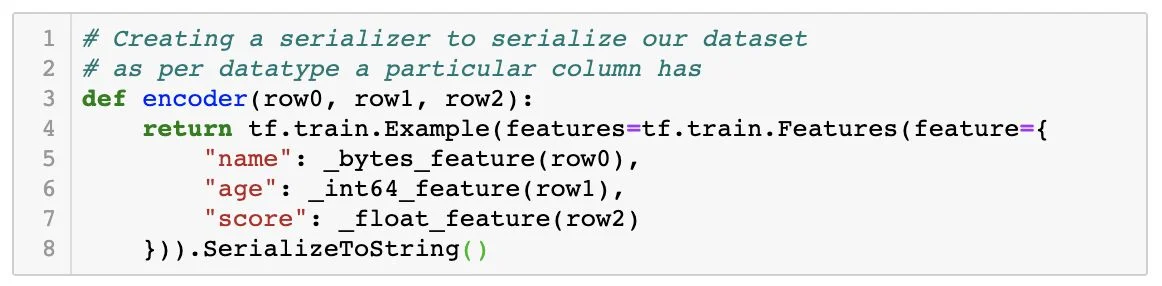
\includegraphics[width=\linewidth,keepaspectratio]{tfdata1}
\end{center}
\end{frame}

%%%%%%%%%%%%%%%%%%%%%%%%%%%%%%%%%%%%%%%%%%%%%%%%%%%%%%%%%%%
\begin{frame}[fragile]\frametitle{From BIG Data}
\lstinline|tf.data.TFRecordDataset|

\begin{center}
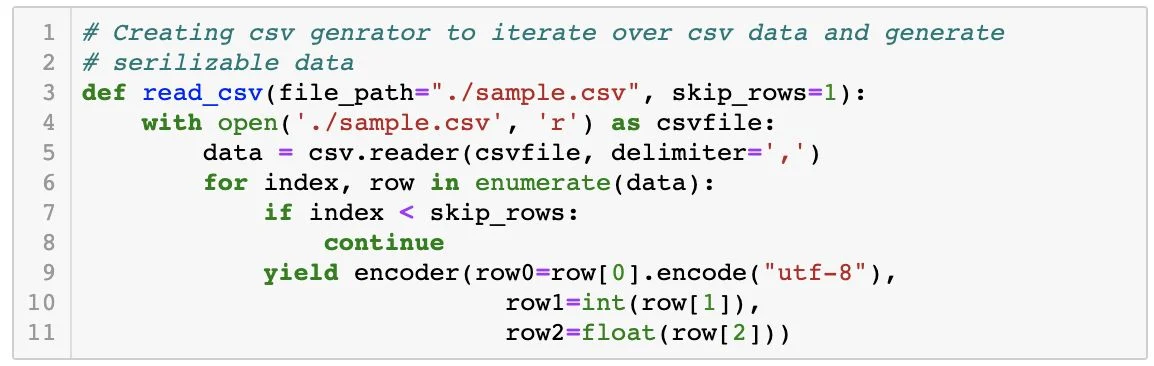
\includegraphics[width=\linewidth,keepaspectratio]{tfdata2}

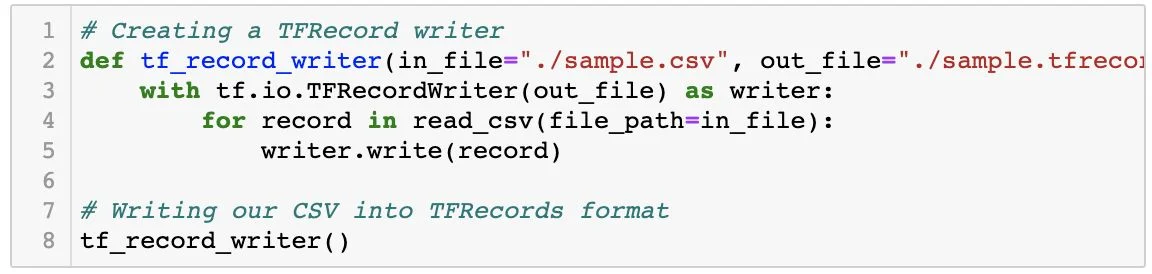
\includegraphics[width=\linewidth,keepaspectratio]{tfdata3}


\end{center}
\end{frame}

%%%%%%%%%%%%%%%%%%%%%%%%%%%%%%%%%%%%%%%%%%%%%%%%%%%%%%%%%%%
\begin{frame}[fragile]\frametitle{From BIG Data}
\lstinline|tf.data.TFRecordDataset|

\begin{center}

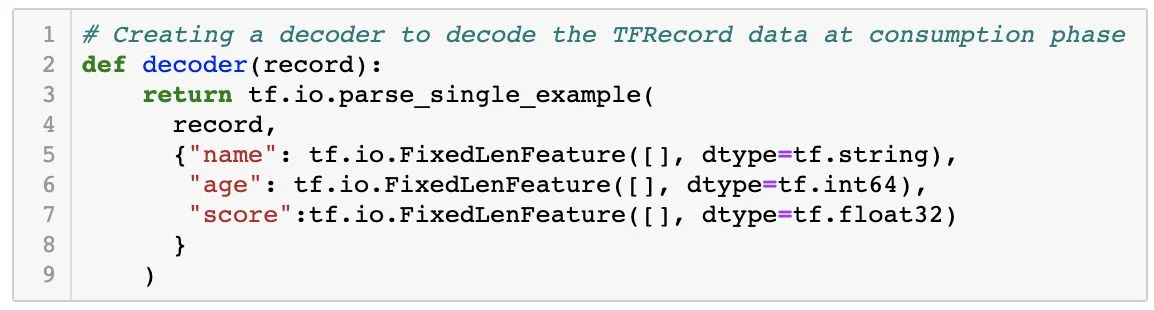
\includegraphics[width=\linewidth,keepaspectratio]{tfdata4}

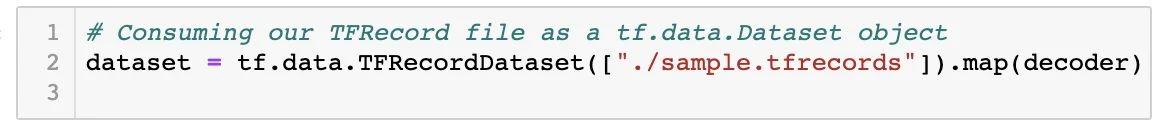
\includegraphics[width=\linewidth,keepaspectratio]{tfdata5}


\end{center}
\end{frame}

%%%%%%%%%%%%%%%%%%%%%%%%%%%%%%%%%%%%%%%%%%%%%%%%%%%%%%%%%%%
\begin{frame}[fragile]\frametitle{Loading text data}

\begin{itemize}
\item Many datasets are distributed as one or more text files. 
\item The tf.data.TextLineDataset provides an easy way to extract lines from one or more text files. 
\item Given one or more filenames, a TextLineDataset will produce one string-valued element per line of those files.
\end{itemize}


\begin{lstlisting}
directory_url = 'https://storage.googleapis.com/download.tensorflow.org/data/illiad/'
file_names = ['cowper.txt', 'derby.txt', 'butler.txt']

file_paths = [
    tf.keras.utils.get_file(file_name, directory_url + file_name)
    for file_name in file_names
]

\end{lstlisting}
\end{frame}

%%%%%%%%%%%%%%%%%%%%%%%%%%%%%%%%%%%%%%%%%%%%%%%%%%%%%%%%%%%
\begin{frame}[fragile]\frametitle{Loading text data}

\begin{itemize}
\item By default, a TextLineDataset yields every line of each file, which may not be desirable, for example, if the file starts with a header line, or contains comments. \item These lines can be removed using the Dataset.skip() or Dataset.filter() transformations. 
\item Here, you skip the first line, then filter to find only survivors.
\end{itemize}


\begin{lstlisting}
dataset = tf.data.TextLineDataset(file_paths)

titanic_file = tf.keras.utils.get_file("train.csv", "https://storage.googleapis.com/tf-datasets/titanic/train.csv")
titanic_lines = tf.data.TextLineDataset(titanic_file)
\end{lstlisting}
\end{frame}


%%%%%%%%%%%%%%%%%%%%%%%%%%%%%%%%%%%%%%%%%%%%%%%%%%%%%%%%%%%
\begin{frame}[fragile]\frametitle{After Dataset}
\begin{itemize}
\item Use \lstinline|.prefetch()| to send next batch data to GPUs or TPUs while current batch is getting completed
\item Use \lstinline|.interleave()| with parallelism for transformation of the dataset, if transformation is needed at the time of consumption phase. 
\item Use \lstinline|.cache()| to cache some computations like transformation which may be overlapping during each epoch.
\end{itemize}


\end{frame}

%%%%%%%%%%%%%%%%%%%%%%%%%%%%%%%%%%%%%%%%%%%%%%%%%%%%%%%%%%%
\begin{frame}[fragile]\frametitle{After Dataset}


\begin{center}
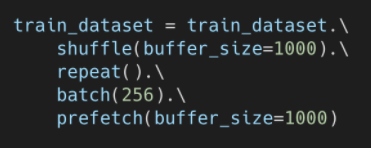
\includegraphics[width=0.6\linewidth,keepaspectratio]{tfdata7}

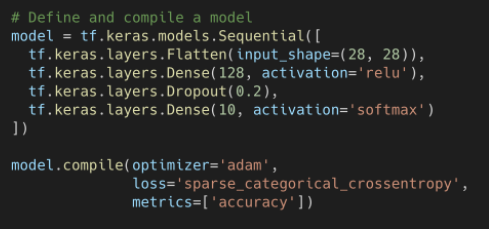
\includegraphics[width=0.6\linewidth,keepaspectratio]{tfdata8}


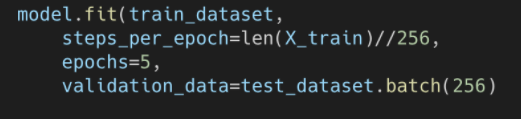
\includegraphics[width=0.6\linewidth,keepaspectratio]{tfdata9}

{\tiny (Ref: Building data pipelines with tf.data - Sayak Paul)}

\end{center}
\end{frame}




%%%%%%%%%%%%%%%%%%%%%%%%%%%%%%%%%%%%%%%%%%%%%%%%%%%%%%%%%%
\begin{frame}
  \begin{center}
    {\Large TensorFlow Data with Image Data Generator}
	
{\tiny (Ref: Building data pipelines with tf.data - Sayak Paul)}

  \end{center}
\end{frame}

%%%%%%%%%%%%%%%%%%%%%%%%%%%%%%%%%%%%%%%%%%%%%%%%%%%%%%%%%%%
\begin{frame}[fragile]\frametitle{Loading Images}

\begin{center}
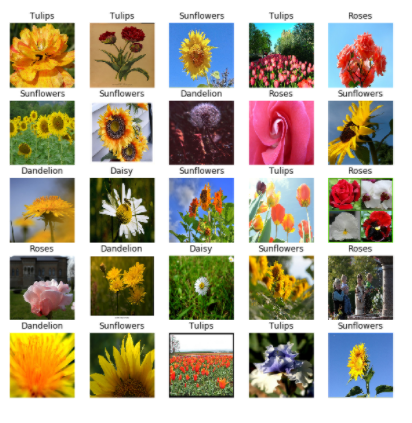
\includegraphics[width=0.4\linewidth,keepaspectratio]{tfdata10}

{\tiny (Ref: Building data pipelines with tf.data - Sayak Paul)}

\end{center}
\end{frame}

%%%%%%%%%%%%%%%%%%%%%%%%%%%%%%%%%%%%%%%%%%%%%%%%%%%%%%%%%%%
\begin{frame}[fragile]\frametitle{ImageDataGenerator}

Initialize ImageDataGenerator with the augmentations.

\begin{center}
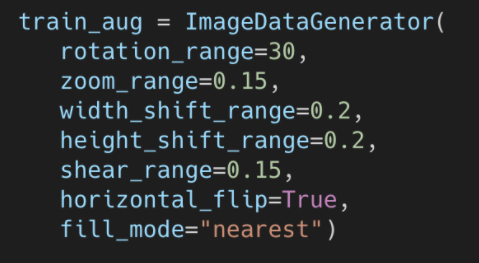
\includegraphics[width=0.6\linewidth,keepaspectratio]{tfdata11}

{\tiny (Ref: Building data pipelines with tf.data - Sayak Paul)}

\end{center}
\end{frame}

%%%%%%%%%%%%%%%%%%%%%%%%%%%%%%%%%%%%%%%%%%%%%%%%%%%%%%%%%%%
\begin{frame}[fragile]\frametitle{tf.data}

Initialize TF Dataset from directory of files (see ``train\_aug'' from ImageDataGenerator)

\begin{center}
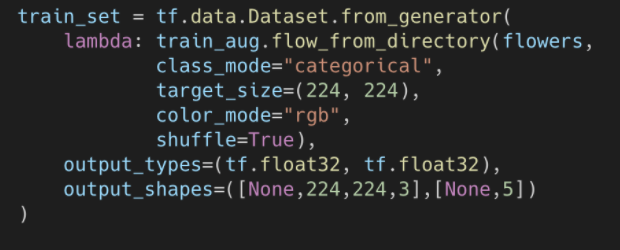
\includegraphics[width=0.6\linewidth,keepaspectratio]{tfdata12}

{\tiny (Ref: Building data pipelines with tf.data - Sayak Paul)}

\end{center}
\end{frame}

%%%%%%%%%%%%%%%%%%%%%%%%%%%%%%%%%%%%%%%%%%%%%%%%%%%%%%%%%%%
\begin{frame}[fragile]\frametitle{Image Preprocessing}

\begin{lstlisting}
list_ds = tf.data.Dataset.list_files(str(flowers_root/'*/*'))

# Reads an image from a file, decodes it into a dense tensor, and resizes it
# to a fixed shape.
def parse_image(filename):
  parts = tf.strings.split(filename, os.sep)
  label = parts[-2]

  image = tf.io.read_file(filename)
  image = tf.image.decode_jpeg(image)
  image = tf.image.convert_image_dtype(image, tf.float32)
  image = tf.image.resize(image, [128, 128])
  return image, label
	
file_path = next(iter(list_ds))
image, label = parse_image(file_path)

def show(image, label):
  plt.figure()
  plt.imshow(image)
  plt.title(label.numpy().decode('utf-8'))
  plt.axis('off')

show(image, label)
\end{lstlisting}
\end{frame}

%%%%%%%%%%%%%%%%%%%%%%%%%%%%%%%%%%%%%%%%%%%%%%%%%%%%%%%%%%%
\begin{frame}[fragile]\frametitle{Image Preprocessing}

If you want to apply a random rotation, the tf.image module only has tf.image.rot90, which is not very useful for image augmentation.

\begin{lstlisting}
def tf_random_rotate_image(image, label):
  im_shape = image.shape
  [image,] = tf.py_function(random_rotate_image, [image], [tf.float32])
  image.set_shape(im_shape)
  return image, label
	
rot_ds = images_ds.map(tf_random_rotate_image)

for image, label in rot_ds.take(2):
  show(image, label)
\end{lstlisting}
\end{frame}

%%%%%%%%%%%%%%%%%%%%%%%%%%%%%%%%%%%%%%%%%%%%%%%%%%%%%%%%%%%
\begin{frame}[fragile]\frametitle{Time series windowing}
\begin{lstlisting}
range_ds = tf.data.Dataset.range(100000)
batches = range_ds.batch(10, drop_remainder=True)
for batch in batches.take(5):
  print(batch.numpy())
	
[0 1 2 3 4 5 6 7 8 9]
[10 11 12 13 14 15 16 17 18 19]
[20 21 22 23 24 25 26 27 28 29]
[30 31 32 33 34 35 36 37 38 39]
[40 41 42 43 44 45 46 47 48 49]
\end{lstlisting}
\end{frame}

%%%%%%%%%%%%%%%%%%%%%%%%%%%%%%%%%%%%%%%%%%%%%%%%%%%%%%%%%%%
\begin{frame}[fragile]\frametitle{Time series windowing}

To make dense predictions one step into the future, you might shift the features and labels by one step relative to each other:

\begin{lstlisting}
def dense_1_step(batch):
  # Shift features and labels one step relative to each other.
  return batch[:-1], batch[1:]

predict_dense_1_step = batches.map(dense_1_step)

for features, label in predict_dense_1_step.take(3):
  print(features.numpy(), " => ", label.numpy())
	
[0 1 2 3 4 5 6 7 8]  =>  [1 2 3 4 5 6 7 8 9]
[10 11 12 13 14 15 16 17 18]  =>  [11 12 13 14 15 16 17 18 19]
[20 21 22 23 24 25 26 27 28]  =>  [21 22 23 24 25 26 27 28 29]
\end{lstlisting}
\end{frame}

%%%%%%%%%%%%%%%%%%%%%%%%%%%%%%%%%%%%%%%%%%%%%%%%%%%%%%%%%%%
\begin{frame}[fragile]\frametitle{Time series windowing}

To predict a whole window instead of a fixed offset you can split the batches into two parts:


\begin{lstlisting}
batches = range_ds.batch(15, drop_remainder=True)

def label_next_5_steps(batch):
  return (batch[:-5],   # Take the first 5 steps
          batch[-5:])   # take the remainder

predict_5_steps = batches.map(label_next_5_steps)

for features, label in predict_5_steps.take(3):
  print(features.numpy(), " => ", label.numpy())
	
[0 1 2 3 4 5 6 7 8 9]  =>  [10 11 12 13 14]
[15 16 17 18 19 20 21 22 23 24]  =>  [25 26 27 28 29]
[30 31 32 33 34 35 36 37 38 39]  =>  [40 41 42 43 44]
\end{lstlisting}
\end{frame}

%%%%%%%%%%%%%%%%%%%%%%%%%%%%%%%%%%%%%%%%%%%%%%%%%%%%%%%%%%%
\begin{frame}[fragile]\frametitle{Time series windowing}

To allow some overlap between the features of one batch and the labels of another, use Dataset.zip:



\begin{lstlisting}
feature_length = 10
label_length = 5

features = range_ds.batch(feature_length, drop_remainder=True)
labels = range_ds.batch(feature_length).skip(1).map(lambda labels: labels[:-5])

predict_5_steps = tf.data.Dataset.zip((features, labels))

for features, label in predict_5_steps.take(3):
  print(features.numpy(), " => ", label.numpy())
	
[0 1 2 3 4 5 6 7 8 9]  =>  [10 11 12 13 14]
[10 11 12 13 14 15 16 17 18 19]  =>  [20 21 22 23 24]
[20 21 22 23 24 25 26 27 28 29]  =>  [30 31 32 33 34]
\end{lstlisting}
\end{frame}

%%%%%%%%%%%%%%%%%%%%%%%%%%%%%%%%%%%%%%%%%%%%%%%%%%%%%%%%%%%
\begin{frame}[fragile]\frametitle{Time series windowing}

Putting this together you might write this function:

\begin{lstlisting}
def make_window_dataset(ds, window_size=5, shift=1, stride=1):
  windows = ds.window(window_size, shift=shift, stride=stride)

  def sub_to_batch(sub):
    return sub.batch(window_size, drop_remainder=True)

  windows = windows.flat_map(sub_to_batch)
  return windows

ds = make_window_dataset(range_ds, window_size=10, shift = 5, stride=3)

for example in ds.take(10):
  print(example.numpy())
	
[ 0  3  6  9 12 15 18 21 24 27]
[ 5  8 11 14 17 20 23 26 29 32]
[10 13 16 19 22 25 28 31 34 37]
[15 18 21 24 27 30 33 36 39 42]
[20 23 26 29 32 35 38 41 44 47]
[25 28 31 34 37 40 43 46 49 52]
[30 33 36 39 42 45 48 51 54 57]
[35 38 41 44 47 50 53 56 59 62]
[40 43 46 49 52 55 58 61 64 67]
[45 48 51 54 57 60 63 66 69 72]
\end{lstlisting}
\end{frame}

%%%%%%%%%%%%%%%%%%%%%%%%%%%%%%%%%%%%%%%%%%%%%%%%%%%%%%%%%%%
\begin{frame}[fragile]\frametitle{Time series windowing}

Then it's easy to extract labels, as before:


\begin{lstlisting}
dense_labels_ds = ds.map(dense_1_step)

for inputs,labels in dense_labels_ds.take(3):
  print(inputs.numpy(), "=>", labels.numpy())
	
[ 0  3  6  9 12 15 18 21 24] => [ 3  6  9 12 15 18 21 24 27]
[ 5  8 11 14 17 20 23 26 29] => [ 8 11 14 17 20 23 26 29 32]
[10 13 16 19 22 25 28 31 34] => [13 16 19 22 25 28 31 34 37]
\end{lstlisting}
\end{frame}

%%%%%%%%%%%%%%%%%%%%%%%%%%%%%%%%%%%%%%%%%%%%%%%%%%%%%%%%%%%
\begin{frame}[fragile]\frametitle{Model Training}

\begin{center}
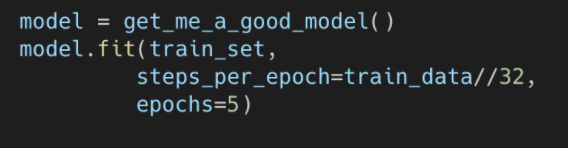
\includegraphics[width=0.6\linewidth,keepaspectratio]{tfdata13}

{\tiny (Ref: Building data pipelines with tf.data - Sayak Paul)}

\end{center}
\end{frame}

%%%%%%%%%%%%%%%%%%%%%%%%%%%%%%%%%%%%%%%%%%%%%%%%%%%%%%%%%%%
\begin{frame}[fragile]\frametitle{Advantages of tf data}
\begin{itemize}
\item It drastically speeds up the data loading time.
\item Fast data loading indeed speeds up the model training. 
\begin{itemize}
\item ImageDataGenerator on the Flowers dataset:
\item tf.data on the Flowers dataset:
\end{itemize}
\end{itemize}
\end{frame}

%%%%%%%%%%%%%%%%%%%%%%%%%%%%%%%%%%%%%%%%%%%%%%%%%%%%%%%%%%%
\begin{frame}[fragile]\frametitle{Summary}
Lets get started \ldots

\begin{center}
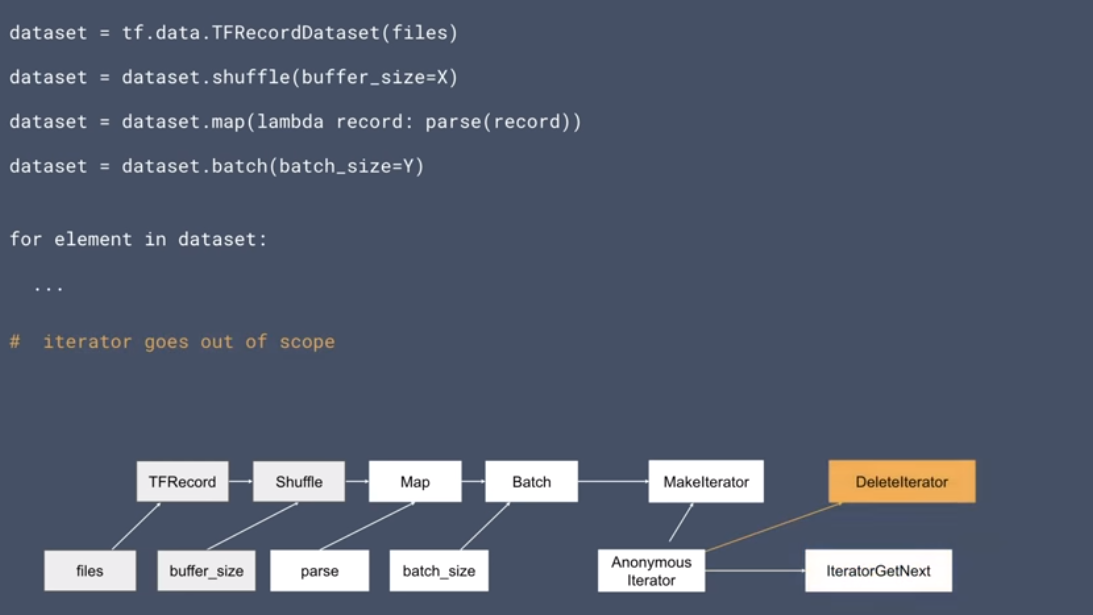
\includegraphics[width=\linewidth,keepaspectratio]{tfdata6}

{\tiny (Ref: Inside TensorFlow: tf.data - TF Input Pipeline )}

\end{center}
\end{frame}